\sect{Аналитическая часть}
\label{cha:A}
В данной части приводится анализ предметной области и формализуются данные и задачи программного обеспечения. Также приводится анализ моделей баз данных.

%=======================================================================================================================
\subsect{Анализ предметной области}
Создание парковочных мест является неотъемлемой частью организации дорожно-транспортной системы. 
Один из самых удобных способов решения этой задачи -- автоматические автопарковки~\cite{actual_autoparking}.
Использование такого типа парковок позволяет не только снизить затраты на организацию инфраструктуры парковок, но и обеспечить круглосуточный сервис для автовладельцев.

Въезд и выезд на такие парковки осуществляется при помощи талонов или  RFID-карт. Оплачивается же время парковки на специальных устройствах~--~паркоматах, поддерживающих оплату как наличными, так и банковской картой.

Как правило, на въезде на парковку стоит табло с указанием количества свободных мест. На самой парковки ведется видеонаблюдение, что повышает безопасность припаркованного транспорта.

%=======================================================================================================================
\subsect{Анализ существующих решений}
Разработка приложения для сети автопарковок позволяет сделать процесс парковки более удобным.
В частности, с помощью приложения возможно организовать бронь парковочного места, получить информацию о количестве свободных мест, оформить абонемент, оплатить время парковки с помощью QR-кода.
Используя перечисленные возможности как критерии, был проведен анализ существующих решений, таких как: 
\begin{itemize}
	\item Came Vector~\cite{came_vector};
	\item Квазар~\cite{kvazar};
	\item Московский паркинг~\cite{parking_Moscow}.
\end{itemize}
Результаты анализа приведены в таблице~\ref{tab:existing_decision}.

\renewcommand{\thetable}{\thesubsection.\arabic{table}}
\begin{table}[H]
	\begin{center}
		\begin{center}
			\caption{\label{tab:existing_decision}Сравнение известных решений}
		\end{center}
		\begin{tabular}{|c|c|c|c|}
			\hline 
			~ & Московский паркинг & Came Vector & Квазар \\ \hline
        Возможность брони & нет & нет & нет \\ \hline
        \specialcell{Информация о количестве \\ свободных мест} & да & да & нет \\ \hline
        Оформление абонемента & да & нет & да \\ \hline
        Оплата с помощью QR-кода & нет & нет & нет \\ \hline
		\end{tabular}
	\end{center}
\end{table}

Как видно из результатов анализа, ни одно из существующих решений не удовлетворяет всем решениям.

%=======================================================================================================================
\subsect{Формализация задача}
В данной курсовой работе необходимо разработать базу данных для хранения информации о парковках и приложение для получения и обработки информации, хранящейся в ней.

%\renewcommand{\thefigure}{\thesubsection.\arabic{figure}}
%\begin{figure}[h]
%	\centering
%	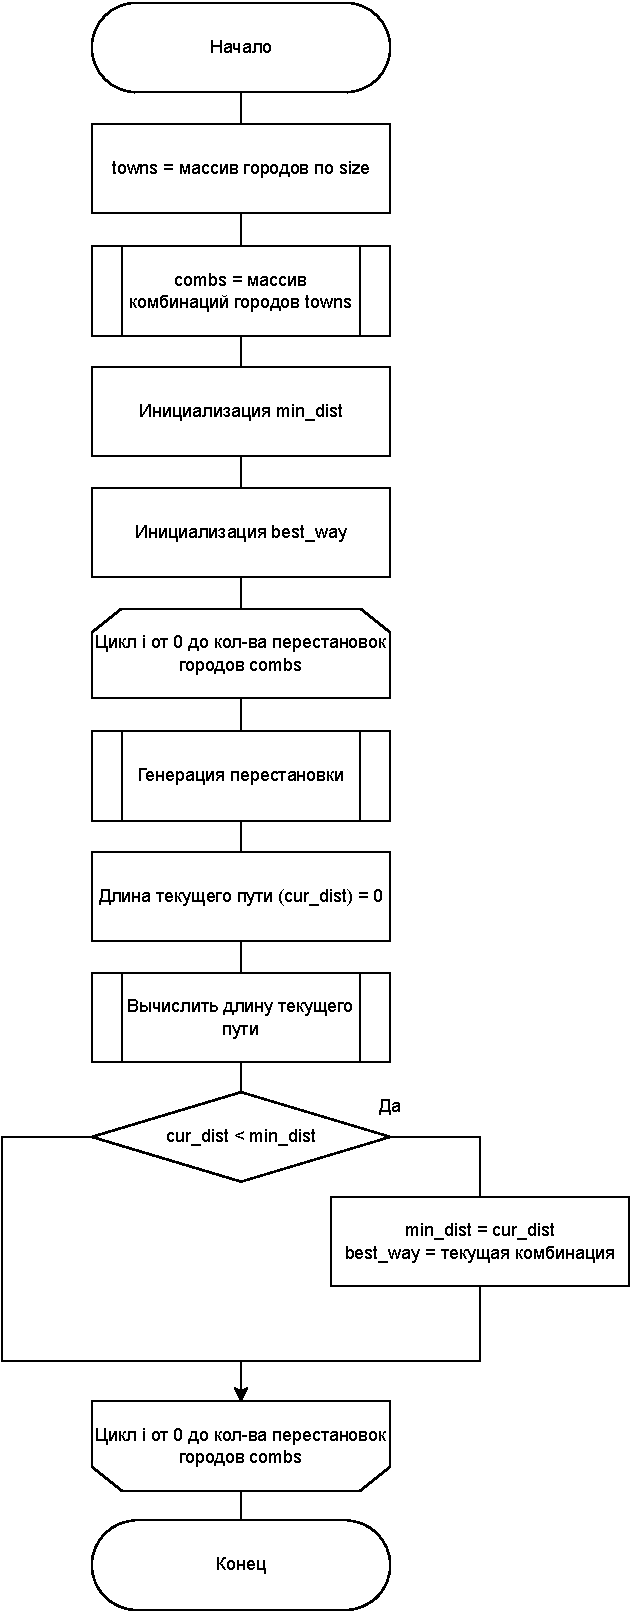
\includegraphics[height=0.9\textheight]{svg/all_combs}
%	\caption{Схема алгоритма полного перебора}
%	\label{fig:full-comb}
%\end{figure}


%=======================================================================================================================
\subsect{Формализация данных}

%=======================================================================================================================
\subsect{Анализ баз данных}

%=======================================================================================================================
\subsect{121}

%=======================================================================================================================
\subsect{121}
